\documentclass[10pt, a4paper, italian]{article}
\usepackage[T1]{fontenc}
\usepackage[utf8]{inputenc}
\usepackage{amsmath, amssymb, amsthm, thmtools, amsfonts, mathtools}
\usepackage{nicefrac}
\usepackage{calc}
\usepackage[pdftex, hyperindex, plainpages=false]{hyperref}
\usepackage[nameinlink]{cleveref} %load before classicthesis (clash)
%\usepackage[nochapters,pdfspacing]{classicthesis}
\usepackage{siunitx}
\usepackage[siunitx]{circuitikz}

\usepackage[a4paper]{geometry}
\usepackage{float}
\usepackage{mdframed}
\usepackage{titling}
\usepackage{booktabs}
\usepackage{graphicx}
\usepackage{caption, subcaption}
\usepackage{xcolor}
\usepackage[italian]{babel}
\usepackage{pgfplots}
\usepackage{listings}
%\usepackage{lmodern}
\usepackage{url}
\usepackage{enumitem}
\usepackage{tikz} %loads after classicthesis (xcolor incompat)

% lets graphicx know path where figures to be included are found
\graphicspath{{../figs/}}
\makeatletter
\def\input@path{{../figs/}}
%or: \def\input@path{{/path/to/folder/}{/path/to/other/folder/}}
\makeatother

% tikz pgf plots setup
\usepgfplotslibrary{external}
\pgfplotsset{compat=1.15}
%\tikzexternalize

% spaces and significant digits/figures for measurements
\sisetup{free-standing-units, space-before-unit, number-unit-product = \;,
scientific-notation = false, round-mode = figures, round-precision = 1,}

% turns all (hyperlinked) references black [default is blue]
\hypersetup{
	linktoc=all,
	colorlinks=true,
	linkcolor=black
}

% code listings config
%\lstset{
%language=Python,
%basicstyle=\ttfamily,
%columns=fullflexible,
%keepspaces=true,
%}

% mdframed (for boxed text) configuration
\mdfsetup{linewidth=0.6pt}

% Default fixed font does not support bold face
\DeclareFixedFont{\ttb}{T1}{txtt}{bx}{n}{12} % for bold
\DeclareFixedFont{\ttm}{T1}{txtt}{m}{n}{12}  % for normal

% Custom colors
\usepackage{color}
\definecolor{deepblue}{rgb}{0,0,0.5}
\definecolor{deepred}{rgb}{0.6,0,0}
\definecolor{deepgreen}{rgb}{0,0.5,0}

% Commands 
\newcommand{\executeiffilenewer}[3]{%
	\ifnum\pdfstrcmp{\pdffilemoddate{#1}}%
		{\pdffilemoddate{#2}}>0%
	{\immediate\write18{#3}}\fi%
}
% input .svg --> .pdf_tex graphs
%\newcommand{\includesvg}[1]{%
%	\executeiffilenewer{#1.svg}{#1.pdf}%
%	{inkscape -z -D --file=#1.svg %
%	--export-pdf=#1.pdf --export-latex}%
%	\input{#1.pdf_tex}%
%}
% Thanks UniPi's Department of Physics E. Fermi
\newcommand{\thanksdf}{(\thanks{Dipartimento di Fisica E.~Fermi,%
Universit\`a di Pisa - Pisa, Italy.}\;)}

% hyperlink to email address
\newcommand{\mail}[1]{\href{mailto:#1}{\textsf{#1}}}

% \vec for bold vectors, instead of overarrows (now "\arrvec")
\let\arrvec=\vec
\renewcommand{\vec}[1]{\boldsymbol #1}
% replaces straight phi with slanted phi
\renewcommand{\phi}{\varphi}
% replaces straight eps with curved epsilon
\newcommand{\eps}{\varepsilon}
% abbreviation for (sub_/super^)scripts of \lim, \sum,... in inline math
\newcommand{\ds}{\displaystyle}

% blackboard/number set letters
\newcommand{\CC}{\mathbb C}
\newcommand{\HH}{\mathbb H}
\newcommand{\KK}{\mathbb K}
\newcommand{\NN}{\mathbb N}
\newcommand{\PP}{\mathbb P}
\newcommand{\QQ}{\mathbb Q}
\newcommand{\RR}{\mathbb R}
\newcommand{\ZZ}{\mathbb Z}

\newcommand{\Abs}[1]{{\left\Vert #1\right\Vert}}
\newcommand{\enclose}[1]{{\left( #1 \right)}}
\newcommand{\Enclose}[1]{{\left[ #1 \right]}}
\newcommand{\floor}[1]{\left\lfloor #1 \right\rfloor}
\newcommand{\ceil}[1]{\left\lceil #1 \right\rceil}
\newcommand{\To}{\rightrightarrows}

% Math operators
\DeclareMathOperator{\divergence}{div}
\renewcommand{\div}{\divergence}
\DeclareMathOperator{\Imaginarypart}{Im}
\renewcommand{\Im}{\Imaginarypart}
\DeclareMathOperator{\Realpart}{Re}
\renewcommand{\Re}{\Realpart}
%\DeclareMathOperator{\arg}{arg}
\DeclareMathOperator{\tg}{tg}
\DeclareMathOperator{\arctg}{arctg}
\DeclareMathOperator{\settsinh}{settsinh}
\DeclareMathOperator{\settcosh}{settcosh}
\DeclareMathOperator{\tr}{tr}
\DeclareMathOperator{\im}{im}
\DeclareMathOperator{\sgn}{sgn}
\DeclareMathOperator{\diag}{diag}

\DeclarePairedDelimiter{\norm}{\lVert}{\rVert}
\DeclarePairedDelimiter{\scalar}{\langle}{\rangle}

% Logarithm with arbitrary base.
% -> log_10
\newcommand{\llog}[1][10]{\log_{#1}}

% Absolute value.
% -> |x|
\newcommand{\abs}[1]{\left| #1 \right|}

% Powers.
% -> x^a
\newcommand{\power}[2][2]{\left( #2 \right)^{#1}}

% Square.
% -> x^2
\newcommand{\sq}[1]{\power[2]{#1}}

% Expansion of the binomial coefficient.
% -> n1!/(n2!(n1 - n2)!)
\newcommand{\binomexpr}[2]{\frac{#1!}{#2!(#1 - #2)!}}

% Expression evaluation at a given point with square brackets.
% -> [x]_{a}
\newcommand{\at}[2]{\left[ #1\right]_{\makebox[-1pt][l]{${\scriptstyle#2}$}}}

% Expression evaluation in an interval.
% -> [x] _{a}^{b}
\newcommand{\eval}[3]{\left.#1%
  \right|_{\makebox[-1pt][l]{${\scriptstyle#2}$}}^{\makebox[-1pt][l]{${\scriptstyle#3}$}}}

% Upright d in math mode (for differentials).
% -> d
\newcommand{\ud}{\mathrm{d}}

% Differential.
% -> dx
\newcommand{\diff}[1][x]{\,\ud{#1}}

% Base command for defining derivatives.
% -> df/dx or d^kf/dx^k
\newcommand{\basederivative}[4][]{%
  \displaystyle%
  \ifx\\#1\\\frac{#4#2}{#4#3}%
  \else%
  \frac{#4^#1#2}{#4#3^#1}%
  \fi%
}

% Total derivative.
% -> df/dx(x) or d^kf/dx^k(x)
\newcommand{\td}[4][]{%
  \basederivative[#1]{#2}{#3}{\ud}%
  \ifx\\#4\\%
  \else%
  \mkern-4mu\left(#4\right)%
  \fi%
}

% Partial derivative.
% -> df/dx(x) or d^kf/dx^k(x)
\newcommand{\pd}[4][]{%
  \basederivative[#1]{#2}{#3}{\partial}%
  \ifx\\#4\\%
  \else%
  \mkern-4mu\left(#4\right)%
  \fi%
}

\newcommand{\intinf}{\int_{-\infty}^{\infty}\!\!\!}

\newcommand{\cinterval}[2]{\left[\, #1,~#2 \,\right]}

\newcommand{\linterval}[2]{\left[\, #1,~#2 \,\right)}

\newcommand{\rinterval}[2]{\left(\, #1,~#2 \,\right]}

\newcommand{\ointerval}[2]{\left(\, #1,~#2 \,\right)}

\newcommand{\prob}[1]{\displaystyle P\left(#1\right)}

\newcommand{\pvalue}{\emph{$p$-value}}

\newcommand{\cond}{\,|\,}

\newcommand{\expect}[1]{\displaystyle E\left[#1\right]}

\newcommand{\mom}[2][]{\displaystyle {\cal M}_{#2}\ifx\\#1\\\else(#1)\fi}

\newcommand{\momalg}[1]{\displaystyle \lambda_{#1}}

\newcommand{\momcen}[1]{\displaystyle \mu_{#1}}

\newcommand{\skewness}{\displaystyle \gamma_1}

\newcommand{\kurtosis}{\displaystyle \gamma_2}

\newcommand{\charf}[1][x]{\phi_{#1}}

\newcommand{\momgenf}[1][x]{M_{#1}}

\newcommand{\fwhm}{{\scriptstyle \textsc{FWHM}}}

\newcommand{\hwhm}{{\scriptstyle \textsc{HWHM}}}

\newcommand{\median}{\mu_{\nicefrac{1}{2}}}

\newcommand{\var}[1]{\ensuremath{\text{Var}\left(#1\right)}}

\newcommand{\cov}[2]{\ensuremath{\text{Cov}\left(#1, #2\right)}}

\newcommand{\corr}[2]{\ensuremath{\text{Corr}\left(#1, #2\right)}}

\newcommand{\like}{\mathcal L}

\newcommand{\likelihood}[2][]{\like\ifx\\#2\\\else(#2\ifx\\#1\\\else;#1\fi)\fi}

\newcommand{\chisq}{\ensuremath{\chi^2}}

\newcommand{\chisquare}[2][]{\chisq\ifx\\#2\\\else(#2\ifx\\#1\\\else;#1\fi)\fi}

\newcommand{\loglikelihood}[2][]{\log\likelihood[#1]{#2}}

\newcommand{\pdf}[3][]{#2(#3\ifx\\#1\\\else;#1\fi)}

\newcommand{\binomialpdf}[2][]{\pdf[#1]{\mathcal B}{#2}}

\newcommand{\multinomialpdf}[2][]{\pdf[#1]{\mathcal M}{#2}}

\newcommand{\poissonpdf}[2][]{\pdf[#1]{\mathcal P}{#2}}

\newcommand{\uniformpdf}[2][]{\pdf[#1]{u}{#2}}

\newcommand{\exponentialpdf}[2][]{\pdf[#1]{\varepsilon}{#2}}

\newcommand{\gausspdf}[2][]{\pdf[#1]{N}{#2}}

\newcommand{\chisquarepdf}[2][]{\pdf[#1]{\wp}{#2}}

\newcommand{\cauchypdf}[2][]{\pdf[#1]{c}{#2}}

\newcommand{\erf}[1]{\ensuremath{\text{erf}\left(#1\right)}}

\newcommand{\dccases}[4][]{#2 \ifx\\#2\\\else=\fi %
  \begin{cases}
    \displaystyle #3 & \text{per variabili discrete}\\
    \displaystyle #4 & \text{per variabili continue}#1
  \end{cases}
}
% sub/super-scriptable for all symbol as math operator 
\newcommand\Scaleforall[1]{\vcenter{\hbox{\scalefont{#1}$\forall$}}}

\DeclareMathOperator*\forevery{%
  \vphantom\sum
  \mathchoice{\Scaleforall{2}}{\Scaleforall{1.4}}{\Scaleforall{1}}{\Scaleforall{0.75}}}
\geometry{left=2cm, right=2cm, top=2cm, bottom=2cm}

% indexes subsections with letters, sections with numbers (1.a, 1.b, ...)
\renewcommand{\thesubsection}{\thesection.\alph{subsection}}

% lets graphicx know path where figures to be included are found
\graphicspath{{../figs/}}

\author{Gruppo 1.AC \\ Matteo Rossi, Bernardo Tomelleri}
\title{Es11: Esperimenti di Interferometria per misure di lunghezze d'onda}
\begin{document}
\date{\today}
\maketitle

%=======================
\section{Scopo dell'esperienza}
Lo scopo dell'esperienza è misurare la lunghezza d'onda di un laser
a semiconduttore studiando il pattern di diffrazione generato da un suo
fascio incidente sulla scala millimetrata di un calibro.

\section{Descrizione della misura}
Dalla teoria sulla natura ondulatoria della luce sappiamo che quando un'onda incide su un reticolo di diffrazione viene diffratta in diversi fasci: il fascio di luce che non subisce deviazioni e che viene trasmesso direttamente viene chiamato ordine 0, che può essere individuato sullo schermo come il punto di massima luminosità. Se poi andiamo a calcolare l'angolo di diffrazione degli altri fasci di luce deviati rispetto a un punto di riferimento, e considerando che i raggi vengono anche riflessi dal nostro reticolo, possiamo stabilire un relazione che collega la posizione dei massimi di rifrazione con la lunghezza d'onda $\lambda$, gli angoli degli ordini di diffrazione $\theta _m$, il passo del reticolo $d$ e l'angolo di incidenza sul reticolo $\theta _i$
\begin{equation}
d(\sin(\theta _i) - \sin(\theta _m))=m \lambda
\label{eq:diff}
\end{equation}
Possiamo dunque riscrivere l'equazione \ref{eq:diff} come:
\begin{equation}
Y= -X \frac{\lambda}{d} +Q
\label{eq:fit}
\end{equation}
dove Y,X e Q sono rispettivamente $\sin(\theta _m)$, m e $\sin(\theta _i)$; da cui si riconosce subito l'equazione di una retta, con coefficiente angolare $\frac{\lambda}{d}$.
\begin{figure}
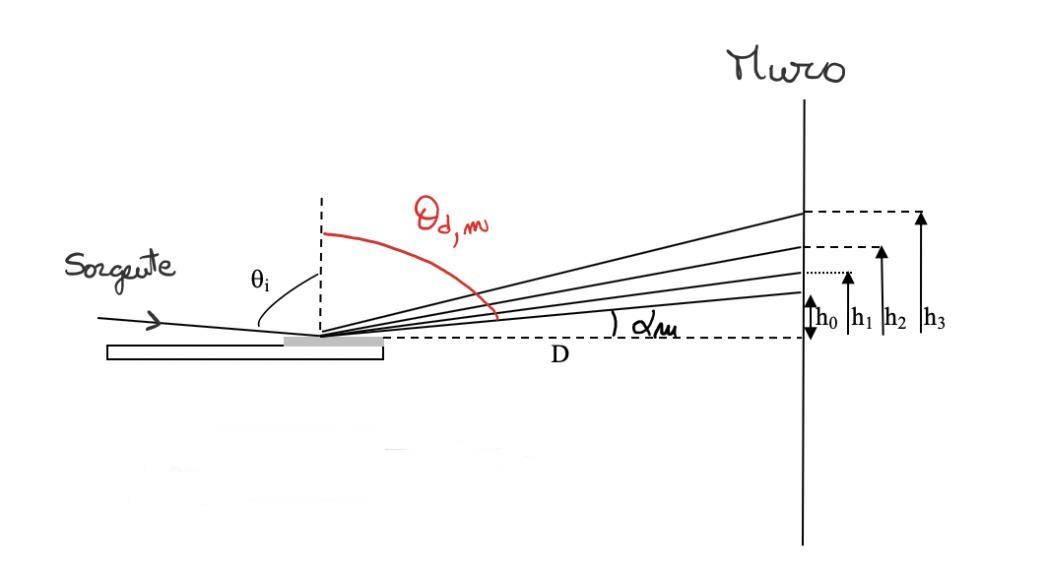
\includegraphics[width=\textwidth]{0}
\caption{ \label{schema1} Schema di riferimento dell'apparato sperimentale utilizzato}
\end{figure}
Per determinare gli angoli $\theta _m$ dei vari fasci è sufficiente utilizzare la definizione di $\sin$ per arrivare alla conclusione che
\begin{equation}
\sin(\theta _m)=\frac{D}{\sqrt{D^2 + h_m^2}}=(1+ (\frac{h_m}{D})^2)^{-\frac{1}{2}}
\label{eq:gon}
\end{equation}
dove $h_m$ sono le altezze relative dei massimi di diffrazione rispetto al punto di riferimento (nel nostro caso sarà l'altezza a cui si trova il calibro).
\subsection{Apparato}
Utilizzeremo un diodo laser con una lunghezza d'onda pari a 636.4 nm.
Come reticolo di diffrazione abbiamo utilizzato la superficie riflettente di un calibro (quindi con passo $d=1 \; mm$).
Utilizzando lo schema in figura \ref{schema1} abbiamo cominciato misurando la distanza tra lo schermo e il punto d'incidenza del fascio luminoso sul calibro:
\[
D=2.90 \pm 0.03 m
\]
il valore dell'incertezza deriva dal fatto che il punto preciso in cui il fascio laser incide sul calibro è difficile da stimare, perché invece di un punto si osserva una regione luminosa lunga circa 6 cm (d'altronde $\theta _i$ è molto vicino a $\pi /2$), di conseguenza abbiamo preso come errore la semilarghezza dello spot luminoso.
Successivamente abbiamo spostato il calibro in modo che solo una porzione del fascio incidesse sulla scala del calibro, mentre il restante continuasse la sua traiettoria rettilinea senza essere riflesso.
Abbiamo ottenuto così un'immagine da cui si potesse stimare il piano di riferimento da cui far partire le misure di $h_m$ prendendo il punto medio tra il punto dove incideva il fascio riflesso, e il punto in cui incideva il fascio "diretto"; da qui abbiamo stimato il valore di $h_0$:
\[
h_0=5.7 \pm 0.1 cm
\]
per concludere le misure abbiamo registrato le altezze di 25 massimi di diffrazione rispetto al piano di riferimento, ognuno con la relativa incertezza (derivata dallo spessore non trascurabile dei singoli spot luminosi).
Utilizzando poi l'equazione \ref{eq:gon} abbiamo stimato i corrispettivi $\sin(\theta _m)$.
\begin{table}[]
\centering
\begin{tabular}{cc|cc}
\toprule
$h_m [cm]$ & $\sigma h_m [mm]$ & $\sin(\theta _m)$ & $\sigma \sin(\theta _m)$\\
\midrule
5,7 & 1 & 1.00& 8 E-06\\
12,2 & 1 & 9,99E-01 & 2 E-05 \\
16,3 & 1 & 9,98E-01 & 4 E-05 \\
19,5 & 1 & 9,98E-01 & 5 E-05 \\
22,3 & 1 & 9,97E-01 & 7 E-05 \\
24,8 & 1 & 9,96E-01 & 8 E-05 \\
27,1 & 2 & 9,96E-01 & 1 E-04 \\
29,2 & 2 & 9,95E-01 & 1 E-04 \\
31,2 & 2 & 9,94E-01 & 1 E-04 \\
33,0 & 2 & 9,94E-01 & 2 E-04 \\
34,7 & 2 & 9,93E-01 & 2 E-04 \\
36,3 & 2 & 9,92E-01 & 2 E-04 \\
37,9 & 2 & 9,92E-01 & 2 E-04 \\
39,4 & 2 & 9,91E-01 & 2 E-04 \\
40,9 & 2 & 9,90E-01 & 2 E-04 \\
42,4 & 3 & 9,89E-01 & 3 E-04 \\
43,7 & 3 & 9,89E-01 & 3 E-04 \\
45,1 & 3 & 9,88E-01 & 3 E-04 \\
46,4 & 3 & 9,87E-01 & 3 E-04 \\
47,7 & 2 & 9,87E-01 & 3 E-04 \\
48,9 & 2 & 9,86E-01 & 3 E-04 \\
50,1 & 2 & 9,85E-01 & 3 E-04 \\
51,3 & 2 & 9,85E-01 & 3 E-04 \\
52,4 & 2 & 9,84E-01 & 3 E-04 \\
53,5 & 1 & 9,83E-01 & 3 E-04 \\
54,5 & 1 & 9,83E-01 & 4 E-04
\end{tabular}
\caption{Dati dei vari $h_m$ (in ordine a partire dall'ordine 0) e dei corrispettivi angoli \label{hm}}
\end{table}



A questo punto tramite un fit lineare $\sin{\theta_m}$ vs $m$ partendo dall'equazione \ref{eq:fit} è possibile stimare il parametro $\frac{\lambda}{d}$ e dunque $\lambda$; nel fare il fit abbiamo escluso il punto $h_0$ per vedere se Q fosse compatibile col suo valore.
\begin{figure}
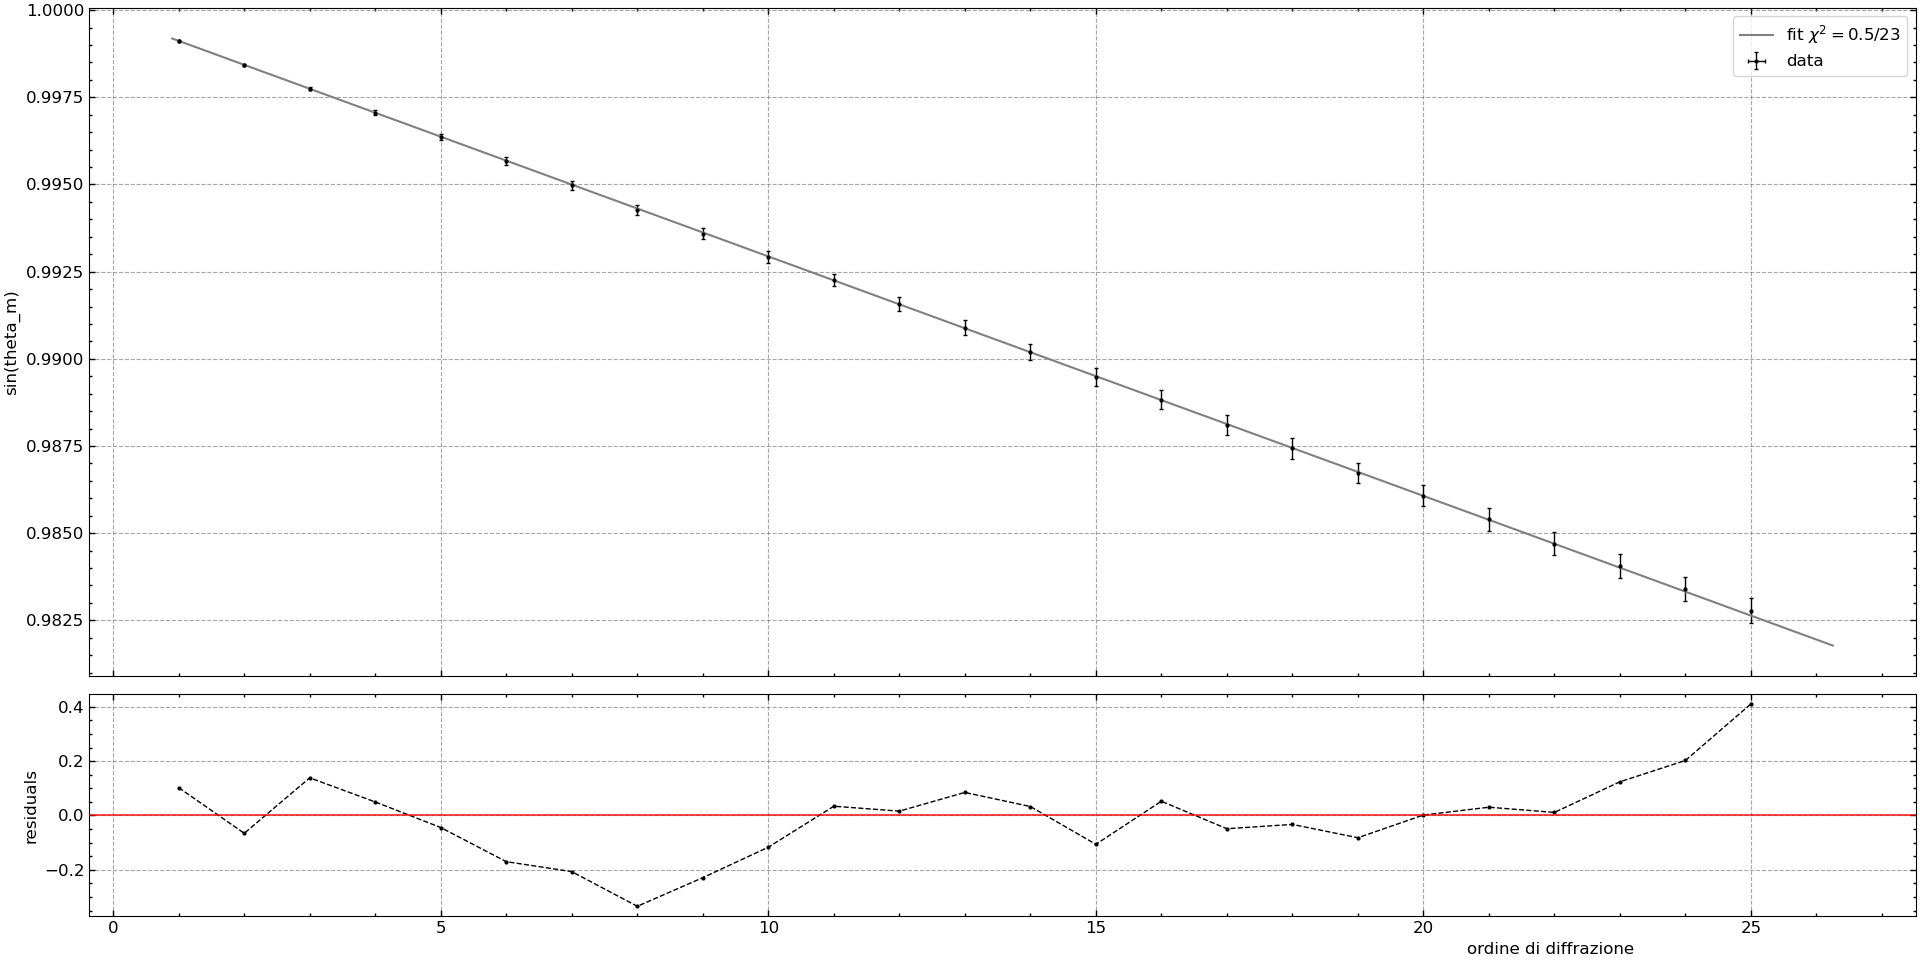
\includegraphics[width=\textwidth]{fit1}
\caption{\label{linfit1} Fit lineare con modello \ref{eq:fit}}
\end{figure}
Dal fit si ricava $\frac{\lambda}{d}=6.87 \pm 0.01 \;\times 10^{-4} \; m$ e $\sin(\theta _i) =1.00 \pm (3 \times 10^{-6})\;$, da cui si ottiene $\lambda=687 \pm 1 \;nm$.
Deduciamo quindi che $\sin(\theta _i)$ è compatibile con quanto ci aspettavamo, invece per quanto riguarda il valore di $\lambda$ possiamo affermare che siamo riusciti a stimare l'ordine di grandezza della lunghezza d'onda, senza però ricavare un valore compatibile con le aspettative; inoltre il grafico dei residui non rivela nessun andamento particolare, quindi non abbiamo ragione per rigettare il modello.
%=======================
\section{Interferometro di Michelson: lunghezza d'onda lampada Hg}
\subsection{Stima del fattore di demoltiplica}
Per calibrare l'apparato e stimare il fattore di demoltiplica della vite-specchio M1 è stato utilizzato un laser He-Ne di lunghezza d'onda nota ($632.8 nm$).
Per prima cosa è stato necessario calibrare lo specchio M2 in modo che sullo schermo appaia un pattern circolare di interferenza dovuto allo sfasamento dei 2 fasci di luce prodotti dalle lenti dell'interferometro.
Una volta posizionato M2 nella posizione corretta abbiamo iniziato a variare la posizione di M1 contando il numero di fronti d'onda passanti da un punto qualunque fisso sullo schermo (per comodità il centro) in funzione dello spostamento effettuato dalla vite di M1. Da qui abbiamo utilizzato l'equazione :
\begin{equation}
\eta= \frac{m \lambda}{2 \Delta L}
\label{dem}
\end{equation}

per ricavare il fattore di demoltiplica $\eta$.
Ripetendo la misura 2 volte abbiamo ottenuto 
  \[
\def\arraystretch{1.5}
\begin{array}{rcl}
\eta_1 & = & 198 \pm 9 \times 10^{-3}\\
\eta_2 & = & 0.21 \pm 0.01\\
\end{array}
\]
facendo poi la media pesata delle misure si ricava $\eta_M =206 \pm 8 \; \times 10^{-3}$.

\subsubsection{Misura della lunghezza d'onda della lampada Hg}
Modificando l'equazione \ref{dem} si giunge a trovare una formula per la stima della lunghezza d'onda in funzione del numero dei fronti d'onda, del fattore di demoltiplica e dello spostamento effettuato dalla vite micrometrica.
\[
\lambda=\frac{2\Delta L \eta}{m}
\]
Abbiamo quindi sostituito la sorgente di radiazione luminosa con una lampada al mercurio di lunghezza d'onda $\lambda=546 nm$; dopodiché utilizzando la stessa procedura di prima abbiamo contato i fronti d'onda in funzione dello spostamento della vite micrometrica.
  \[
\def\arraystretch{1.5}
\begin{array}{rcl}
\lambda_1 & = & 5.5 \pm 0.4 \times 10^{-7} m\\
\lambda_2 & = & 5.4 \pm 0.4 \times 10^{-7} m\\
\end{array}
\]
facendo quindi la media pesata si ricava $\lambda _{Hg}=545\pm 28 \; nm$ che risulta totalmente compatibile con le aspettative
%=======================
\section*{Conclusioni e commenti finali}
In quest'esperienza è stato possibile determinare con successo la lunghezza d'onda di un laser a semiconduttore utilizzando un calibro come reticolo di diffrazione. Inoltre, utilizzando un interferometro di Michelson è stata stimata la lunghezza d'onda della riga verde di una lampada a mercurio. Nonostante alcune difficoltà incontrate in quest'ultima stima e le sorgenti di errore abbastanza rilevanti, è stato possibile ottenere una stima compatibile con il valore atteso.

%=======================
\section*{Dichiarazione}
I firmatari di questa relazione dichiarano che il contenuto della relazione \`e
originale, con misure effettuate dai membri del gruppo, e che tutti i firmatari
hanno contribuito alla elaborazione della relazione stessa.


\end{document}